\section{Arrays}\label{sec:array}

An array is a collection of elements. Each element in an array has a position and orientation in the array frame. The array itself also has a position and orientation in the body frame. Sonar Workbench supports arrays with mixed element types, e.g. vector sensor arrays with a mix of hydrophones (omnidirectional elements) and accelerometers (cosine elements). The array structure has fields which contain this information.

The field \texttt{.Ne} holds the integer number of elements in the array. The position, orientation, and element type fields are all column vectors of length \texttt{Ne}. The user is free to choose any convenient element order, as long as that order is consistent across all fields. Three vectors determine the element positions in the array frame, \texttt{.ex}, \texttt{.ey}, and \texttt{.ez}, all in units of meters. Three additional vectors determine the element orientations in the array frame, \texttt{.egamma}, \texttt{.etheta}, and \texttt{.epsi}, corresponding to roll, pitch, and yaw, in degrees.

The array structure holds an additional 6 fields with scalars corresponding to the array position and orientation in the body frame. These fields are \texttt{.ax}, \texttt{.ay}, \texttt{.az}, \texttt{.agamma}, \texttt{.atheta}, and \texttt{.apsi}, in units of meters and degrees. Table~\ref{tab:ArrayFields} summarizes the fields in the array structure. 

\begin{table}[!ht]
	\begin{center}
		\caption{Array structure fields}
		\label{tab:ArrayFields}
		\begin{tabular}{c|l} 
			\textbf{Field} & \textbf{Description} \\
			\hline
			\texttt{.Ne} & number of elements \\
			\texttt{.ex} & element $x$ position vector (m) \\
			\texttt{.ey} & element $y$ position vector (m) \\
			\texttt{.ez} & element $z$ position vector (m) \\
			\texttt{.egamma} & element roll orientation vector ($^\circ$) \\
			\texttt{.etheta} & element pitch orientation vector ($^\circ$) \\
			\texttt{.epsi} & element yaw orientation vector ($^\circ$) \\
			\texttt{.eindex} & element type index (optional) \\
			\texttt{.ax} & array $x$ position (m) \\
			\texttt{.ay} & array $y$ position (m) \\
			\texttt{.az} & array $z$ position (m) \\
			\texttt{.agamma} & array roll orientation ($^\circ$) \\
			\texttt{.atheta} & array pitch orientation ($^\circ$) \\
			\texttt{.apsi} & array yaw orientation ($^\circ$) \\
		\end{tabular}
	\end{center}
\end{table}

\subsection{Arrays with uniform element types}

When all the array elements are identical, the array structure does not need the \texttt{.eindex} field. An example array structure is found in \texttt{SampleArray.m}, shown in Listing~\ref{lst:SampleArray}.

\lstinputlisting[caption={\texttt{SampleArray.m}},label={lst:SampleArray}]{../../examples/SampleArray.m}

This planar array contains 50 rectangular elements arranged in a grid 5 elements wide by 10 elements high. The geometry is shown in \figname~\ref{fig:SampleArray}, with elements numbered according to their order in the array structure.

\begin{figure}[!ht]
\begin{center}
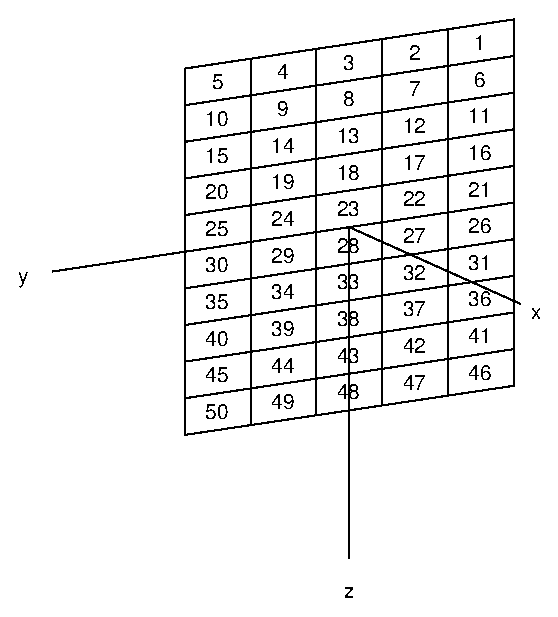
\includegraphics[width=3in]{SampleArray}
\caption{\label{fig:SampleArray}Example rectangular planar array}
\end{center}
\end{figure}

\clearpage
\subsection{Arrays with mixed element types}

For mixed-element arrays, the \texttt{.eindex} field must be a column vector of length \texttt{Ne} integers. The user must first define an element structure array, with one entry for each unique element type. The \texttt{.eindex} field for each element must contain the index into the element structure array corresponding to its element type. 

An example is included in \texttt{SampleVSCardioid.m} for a simple vector sensor. The relevant portion is shown in Listing~\ref{lst:SampleVSCardioid}. This vector sensor consists of four elements: a hydrophone and three orthogonal accelerometers. The three accelerometers are identical except for their orientations, so there are a total of two unique elements. The hydrophone is \texttt{Element(1)}, and the accelerometer is \texttt{Element(2)}. The array structure is named \texttt{VS}, and the hydrophone is the first element, followed by the $x$, $y$, and $z$ accelerometers. This makes the first entry in \texttt{.eindex} equal to 1 and the rest of the entries equal to 2. Fields \texttt{.psi} and \texttt{.etheta} rotate elements 3 and 4 from the $x$ axis to the $y$ and $z$ axes, respectively.

\lstinputlisting[firstline=6,lastline=28,caption={\texttt{SampleVSCardioid.m}},label={lst:SampleVSCardioid}]{../../examples/SampleVSCardioid.m}
